\documentclass[a4paper, 12pt]{book}
% preamble.tex

\usepackage[utf8]{inputenc}
\usepackage[T1]{fontenc}
\usepackage[english]{babel} % Ho cambiato in italian, supponendo che la maggior parte del testo sia in italiano
\usepackage{amsmath}
\usepackage{amssymb}
\usepackage{graphicx}
\usepackage{hyperref}
\usepackage{geometry}
\usepackage{fontspec} % Utile per Xetex/LuaLaTeX ma mantenuto
\usepackage{booktabs}
\usepackage{amsthm}
\usepackage{enumitem}
\usepackage{caption}
\usepackage{thmtools}
\usepackage{standalone} % Già presente nel tuo elenco
\usepackage{tkz-euclide}
\usepackage{graphicx}
\usepackage[T1]{fontenc}
\usepackage{wesa}

% --- PACCHETTI AGGIUNTI PER LA FORMATTAZIONE ---
\usepackage{parskip}  % Aggiunge spazio tra i paragrafi (stile "blocco")
\usepackage{fancyhdr} % Per intestazioni e piè di pagina personalizzati

% --- IMPOSTAZIONI GEOMETRIA E FONT ---
\geometry{a4paper, margin=1in}

% Configura lo stile 'plain' (usato da \maketitle e \tableofcontents)
% per essere coerente con il piè di pagina
\fancypagestyle{plain}{
    \fancyhf{} % Pulisce
    \cfoot{\thepage} % Mette solo il numero di pagina
    \renewcommand{\headrulewidth}{0pt} % Niente linea su queste pagine
}

% Configurazione Header/Footer per le altre pagine
\pagestyle{fancy}
\fancyhead{} % Pulisce l'intestazione
\fancyfoot{} % Pulisce il piè di pagina
\fancyhead[L]{\nouppercase{\rightmark}} % Nome Sezione a sinistra (o Chapter)
\fancyhead[R]{\nouppercase{\leftmark}}  % Nome Capitolo a destra (o Sezione)
\fancyfoot[C]{\thepage} % Numero di pagina al centro
\renewcommand{\headrulewidth}{0.4pt}
\renewcommand{\footrulewidth}{0pt}


% --- DEFINIZIONI TEOREMI ---
% (Questa parte è cruciale per la tua struttura)
\newtheoremstyle{mythmstyle}%
    {}%
    {}%
    {\itshape}%
    {}%
    {\bfseries}%
    {}%
    { }%
    {\thmname{#1}\thmnumber{ #2}%
    \thmnote{: #3\addcontentsline{toc}{subsubsection}{{\itshape#1}: #3}}. }

% 2. Imposta questo stile come quello ATTUALE
\theoremstyle{mythmstyle}

\newtheorem{theorem}{Th}[section]
\newtheorem{definition}{Def}[section]
\newtheorem{proposition}{Prop}[section]
\newtheorem{corollary}{Cor}[section]
\newtheorem{algorithm}{Alg}[section]
\newtheorem{lemma}{Lemma}[section]
\newtheorem*{remark}{Rem}

% Definizioni utili per il Main file
\newcommand{\inputlesson}[1]{\clearpage\input{#1}\clearpage} % Comando per input lezione
\usepackage[x11names, table]{xcolor}
\usepackage{tikz}
\usetikzlibrary{shapes,fit}
\usetikzlibrary{positioning, arrows.meta, shapes.geometric}
\usepackage{amsmath} % Required for align environment
\usepackage{colortbl}


\begin{document}
\setcounter{chapter}{3}
\chapter[ ]{Week 17-23 November}
\section[Channel models]{Channel models (frequency selective, FIR, flat channel); channel normalization and average symbol energy; vector representation of a SISO FIR channel}

An important thing is the normalization of the channel; people normally make lots of mistakes about this.

We have the model defined in (2.19).
We can model such a channel as
\begin{equation}
c_p(\tau) = \sum_{q=0}^{Q-1} A_q \delta(\tau - \tau_q) \;. \tag{2.19}
\end{equation}

If we don't pay attention, this channel could be amplified. We need to pay attention because the energy of the channel is
$$
\sum |A_q|^2 \;,
$$
which might be greater than 1.

% Riquadro Verde
\begin{tcolorbox}[sharp corners, boxrule=0pt, leftrule=2pt, colframe=green!60!black, colback=green!5, left=5pt, top=3pt, bottom=3pt]
    What's important is the ratio between the noise and the amplification of the channel (which comes from the antenna itself, its directionality etc etc): the gain is in respect to an isotropic antenna.
\end{tcolorbox}

In short, the problem is that we want to separate the gain from the channel response, which is why we write:
\begin{align}
c(\tau) &= \sqrt{G}h(\tau) \tag{2.64} \\
c_b(\tau) &= \sqrt{G}h_b(\tau) \tag{2.65} \\
c[l] &= \sqrt{G}h[l] \tag{2.66}
\end{align}
we'll also impose that:
\begin{equation}
\sum_{l} \mathbb{E}|h[l]|^2 = 1
\end{equation}
the channel gain should always be one.

\begin{remark}[This makes perfect sense]
We know that a generic request on the channel is that
\begin{equation*}
\sum_{l} \mathbb{E} \| \boldsymbol{H}[l] \|_F^2 = N_t N_r
\end{equation*}
here we're in SISO, thus we have only one receiver and one transmitter; it makes perfect sense to request that the sum of the expectations is 1.
\end{remark}


\begin{definition}[Frequency selective model]
The \textbf{frequency selective} is a model in which we have $\sqrt{G}$ then a causal and FIR (Finite Impulsive Response) channel and then noise which is IID and $v[n] \sim \mathcal{N}_{\mathbb{C}}(0, N_0)$.

The output of a generic channel, assuming the normalization we mentioned holds, would be:
\begin{equation}
y[n] = \sqrt{G} \sum_{l} h[l]x[n-l] + v[n] \tag{2.69}
\end{equation}
If the condition of FIR and of causality hold, though, the output can be simplified as:
\begin{equation}
y[n] = \sqrt{G} \sum_{l=0}^{L} h[l]x[n-l] + v[n] \tag{2.70}
\end{equation}
\end{definition}

If we then have $L=0$, the channel is multiplicative and will be called \textbf{flat channel}, giving an output of:
\begin{equation}
y[n] = \sqrt{G}h[0]x[n] + v[n] \tag{2.71}
\end{equation}
all the frequencies are treated the same; we can have this model represent a time variant setup if $h[0]$ actually depends on $n$.

If $L > 0$ the channel exhibits ISI (Inter-Symbol Interference) and since its response will not be flat in frequency, we say that it is \textbf{frequency-selective}.

Symbols are normalized to have an \textbf{average symbol energy}:
\begin{equation}
E_s = \frac{1}{N} \sum_{k=0}^{N-1} \mathbb{E}|x[k]|^2
\end{equation}
We'll see that this specific definition is just the per-block power constraint.
We can also have per-symbol or per-antenna power constraints, from which will follow other constraints on the precoding matrix (see \textcolor{green}{signal power constraints}).

This will allow us to write the SNR as:
\begin{equation}
\text{SNR} = \frac{P_r}{N_0/T} = \frac{G E_s}{N_0},
\end{equation}
where:
\begin{itemize}
    \item $P_r$ is the power of the received signal, which in turn is equal to $P_r = G P_x = G E_s / T$ ($P_x$ is the power of the transmitted signal);
    \item $N_0$ is the covariance of the AWGN.
\end{itemize}
This last relation will turn out to be useful later on (it is literally (4.2), (4.3) and it will be of use to write (4.6), (4.7)...).

If we have a frequency-selective channel, we can give a vector representation of (2.70).
For the channel we'll use a Toeplitz matrix, which is a $N \times (N+L)$ convolution matrix defined as:
\begin{equation}
\boldsymbol{H}_{N, N+L} = 
\begin{bmatrix}
h[L] & \dots & h[0] & 0 & \dots & 0 \\
0 & h[L] & \dots & h[0] & 0 & \vdots \\
\vdots & & \ddots & & \ddots & 0 \\
0 & \dots & 0 & h[L] & \dots & h[0]
\end{bmatrix} \tag{2.72}
\end{equation}
the input signal is consequently defined as:
\begin{equation}
\boldsymbol{x}_{N+L} = 
\begin{bmatrix}
x[-L] \\
\vdots \\
x[-1] \\
x[0] \\
x[1] \\
\vdots \\
x[N-1]
\end{bmatrix} \tag{2.73}
\end{equation}
giving that if the channel noise is $\boldsymbol{v}_N$, we'll have:
\begin{equation}
\boldsymbol{y}_N = [y[0] \dots y[N-1]]^T = \sqrt{G} \boldsymbol{H}_{N, N+L} \boldsymbol{x}_{N+L} + \boldsymbol{v}_N \tag{2.74}
\end{equation}
We can show that whichever $n$-th row in (2.74) is equivalent to (2.70).

This is like if we had a MIMO system: "Vectorized result makes an equivalence between frequency-selective SISO channels and frequency-flat MIMO channel, and may be useful for deriving estimators or equalizers".

\begin{figure}[h]
    \centering
    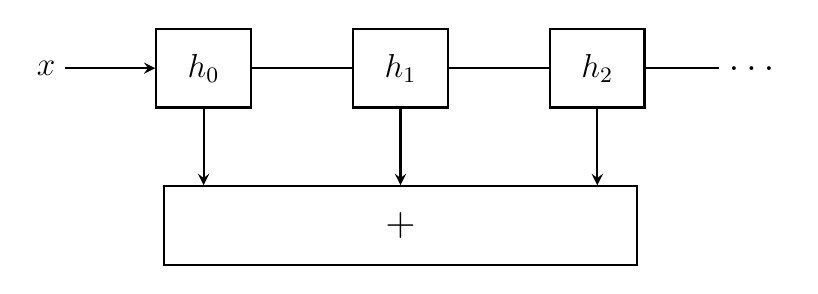
\begin{tikzpicture}[
        node distance=1.5cm,
        block/.style={draw, rectangle, minimum width=1.2cm, minimum height=1cm, align=center, thick},
        sumblock/.style={draw, rectangle, minimum width=6cm, minimum height=1cm, align=center, thick},
        arrow/.style={->, >=stealth, thick}
    ]

    % Input label
    \node (input) at (-2, 0) {\large $x$};

    % Blocchi h0, h1, h2
    \node[block] (h0) at (0,0) {\large $h_0$};
    \node[block] (h1) [right of=h0, node distance=2.5cm] {\large $h_1$};
    \node[block] (h2) [right of=h1, node distance=2.5cm] {\large $h_2$};
    
    % Puntini di sospensione
    \node (dots) [right of=h2, node distance=2cm] {\Large $\dots$};

    % Blocco Sommatore (rettangolo lungo in basso)
    % Posizionato sotto h1 (il centro)
    \node[sumblock] (sum) at (2.5, -2) {\Large $+$};

    % Collegamenti orizzontali (Input -> h0 -> h1 -> h2 -> ...)
    \draw[arrow] (input) -- (h0);
    \draw[thick] (h0) -- (h1);
    \draw[thick] (h1) -- (h2);
    \draw[thick] (h2) -- (dots);

    % Collegamenti verticali verso il sommatore
    % Usiamo le coordinate relative per far atterrare le frecce sul bordo superiore del rettangolo somma
    \draw[arrow] (h0.south) -- (h0 |- sum.north);
    \draw[arrow] (h1.south) -- (h1 |- sum.north);
    \draw[arrow] (h2.south) -- (h2 |- sum.north);

    \end{tikzpicture}
    \caption*{Block diagram of the FIR/Channel model (reconstruction)}
\end{figure}

This is the same of having a MIMO channel with different gains.
We can ask: if we want to estimate a symbol, how can we only get the symbol $x[n]$ we're interested in from $y[n]$?

We'll want to massage the MIMO system to make it similar to our model; we can put together all the matrices and get one only matrix: this is the stacked vector representation.

\section{Organization detour (+mentions of SVD, Precoding)}

Organizational issue: he set up a lecture for next wednesday; this is because on the 1st of November we'll have no lecture.
Professor tried to keep the target so that we could finish before christmas.
We'll also have some other lectures to look over.

One of the next topics is OFDM; he suggests to read the part of the book dealing with it before going through it with lectures; if we read it beforehand, we'll be in a better position.

\paragraph{Lore of the course moment}
About MMSE: when we transmit, this is another way to estimate the symbol transmitted.

Blabbering ab MIMO: if we have $N$ tx and $M$ rx, we have $NM$ paths.

We'll see filters whose coefficients are matrices.

\textbf{Singular value decomposition}: we'll have a specific slide on this.

\textbf{Precoding}: we should try, if possible, to figure what a certain equation means in practice; the antenna may have a main lobe and we can change the main lobe by moving the antenna mechanically.
Precoding is changing the type of transmission without moving the antenna mechanically; we do this using a certain matrix which we call precoding.
With precoding we can steer where the antennas are transmitting.

We'll move to OFDM (used for 4G, 5G and probably will also be used for 6G); we need to see why we use OFDM! That's the wrong approach, since there are other types of modulation (single carrier modulation, just as an example).
When we're transmitting, we have two antennas and a single channel.

We model the channel via spans:
% Inizio del contenuto convertito

% --- Pagina 1 ---

% Riproduzione del diagramma a blocchi (Tx -> Ch -> EQ -> Rx)
\begin{center}
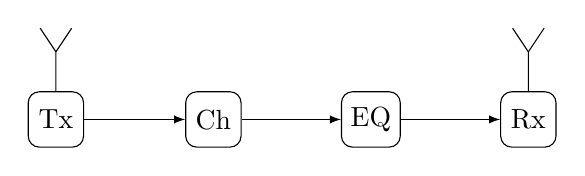
\begin{tikzpicture}[node distance=1.5cm, auto, >=latex]
    % Stile dei blocchi
    \tikzstyle{block} = [draw, rectangle, minimum height=2em, minimum width=2em, rounded corners]
    
    % Nodi
    \node [block] (tx) {Tx};
    \node [coordinate, left of=tx, xshift=0.5cm] (ant_tx_base) {};
    \node [block, right of=tx, node distance=2cm] (ch) {Ch};
    \node [block, right of=ch, node distance=2cm] (eq) {EQ};
    \node [block, right of=eq, node distance=2cm] (rx) {Rx};
    \node [coordinate, right of=rx, xshift=-0.5cm] (ant_rx_base) {};

    % Collegamenti
    \draw [->] (tx) -- (ch);
    \draw [->] (ch) -- (eq);
    \draw [->] (eq) -- (rx);

    % Antenne (stilizzate)
    \draw (tx.north) -- ++(0,0.5) -- ++(-0.2,0.3);
    \draw (tx.north) ++(0,0.5) -- ++(0.2,0.3);
    
    \draw (rx.north) -- ++(0,0.5) -- ++(-0.2,0.3);
    \draw (rx.north) ++(0,0.5) -- ++(0.2,0.3);
\end{tikzpicture}
\end{center}

If we have reflection, the previous signal might superpose to the previous one.
The channel has a non-linear response: we can equalize it!
We have many ways to equalize the channel!

The EQ in MIMO would increase the noise! We thus look at two \textbf{different types of equalizations}; we can have a linear or a non-linear equalization, but the latter is more resource-heavy.

We'll then look at the basics of radio propagation and such; there will be many concepts which are really important and will be pointed out.
We'll see the Friis equation.

% Riquadro Esame (Bordo Rosso)
\noindent\fcolorbox{red}{white}{
    \begin{minipage}{\dimexpr\linewidth-2\fboxsep-2\fboxrule}
        \textcolor{red}{\textbf{$\diamond$ Exam}}
        \vspace{0.5em}
        
        Example of exam question: we can transmit at $900\text{MHz}$ or at $24\text{GHz}$; we have a fixed power $P$ and we can decide which frequency. \\
        Thanks to the Friis equation, we know that choosing the lower frequency is better.
    \end{minipage}
}

The state is getting more money from choosing the higher frequency.

\section[Problems in discretization]{Problems in discretization: multiple paths, multiple taps (+synchronization, reflection and noise whitening)}

We've seen that long time ago people were manipulating analog signals, aka continuous time.
Microphones are still in frequency modulation, as an example.
Long time ago, we were able to communicate and we supposedly went to the moon.

Kalman filtering learned about his filter in Moscow.

We were used at working with analog signals; the leap happened when we began manipulating signals with computers: in order to do this, we need to discretize signals.
Analog circuits are different from one another; computers always do the same operations!
It's much better for us to manipulate signals in a discrete domain!

What if we have a certain channel with a response which is an impulse?

% --- Pagina 2 ---


\section{Discretized Channel Model}

\subsection*{One-tap}

% Grafico Impulso delta(tau)
\begin{center}
\begin{tikzpicture}
    \draw[->] (-2,0) -- (2,0) node[right] {$\tau$};
    \draw[->] (0,0) -- (0,1.5) node[above] {$c(\tau)$};
    \draw[thick] (0,0) -- (0,1);
    \filldraw (0,1) circle (1pt);
\end{tikzpicture}
\end{center}

Whatever is transmitted, it arrives straight to the receiver.
This is true up to a certain point: it might take a while for the signal to travel up to the destination: we might want to move our delta! This is a problem which is called \textbf{time synchronization}.

How can the transmitter understand when $t=0$ is? We might have a form of mismatching if the receiver doesn't understand correctly when the signal started.
We might do syncing using autocorrelation: CAZAC sequences are generally used (Constant Amplitude Zero AutoCorrelation waveform).

Here we suppose that our signal is synchronized; let's convolve it with a sinc; we have that sampling it will give a Kronecker delta function.
\begin{center}
    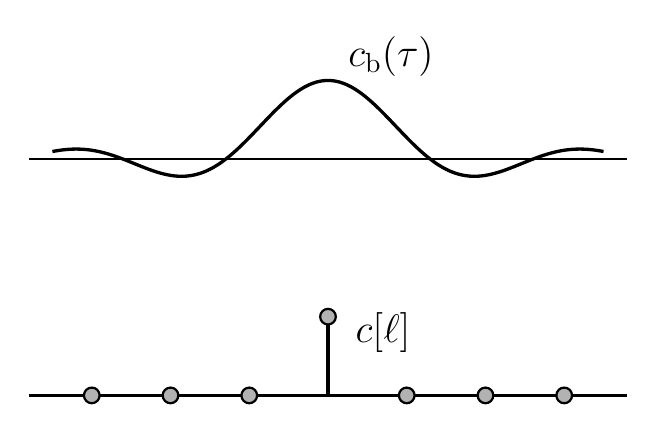
\begin{tikzpicture}
    % Definizione dello stile per i marcatori grigi
    \tikzset{
        marker/.style={
            circle,
            draw=black,
            thick,
            fill=gray!60,
            inner sep=2pt,
            outer sep=0pt
        }
    }

    % --- Grafico Superiore: c_b(\tau) (Continuo) ---
    \begin{scope}[yshift=1.5cm]
        % Asse orizzontale
        \draw[thick] (-3.8, 0) -- (3.8, 0);

        % La curva (funzione sinc approssimata per corrispondere visivamente)
        % Disegnamo in due parti per evitare la divisione per zero a x=0
        \draw[very thick, variable=\t, domain=0.001:3.5, samples=200, smooth]
            plot (\t, {sin(deg(pi*\t/1.3))/(pi*\t/1.3)});
        \draw[very thick, variable=\t, domain=-3.5:-0.001, samples=200, smooth]
            plot (\t, {sin(deg(pi*\t/1.3))/(pi*\t/1.3)});
        % Chiudiamo il piccolo gap centrale al picco
        \draw[very thick] (0,1) -- (0.001, {sin(deg(pi*0.001/1.3))/(pi*0.001/1.3)});
        \draw[very thick] (0,1) -- (-0.001, {sin(deg(pi*-0.001/1.3))/(pi*-0.001/1.3)});

        % Etichetta
        \node at (0.8, 1.3) {\Large $c_{\text{b}}(\tau)$};
    \end{scope}


    % --- Grafico Inferiore: c[l] (Discreto) ---
    \begin{scope}[yshift=-1.5cm]
        % Asse orizzontale
        \draw[thick] (-3.8, 0) -- (3.8, 0);

        % Campioni a zero (punti grigi sull'asse)
        % Assumiamo che i punti siano a coordinate intere
        \foreach \x in {-3, -2, -1, 1, 2, 3} {
            \node[marker] at (\x, 0) {};
        }

        % Impulso centrale (Kronecker delta)
        \draw[very thick] (0, 0) -- (0, 1); % Gambo verticale
        \node[marker] at (0, 1) {};         % Marcatore in cima

        % Etichetta
        \node at (0.7, 0.8) {\Large $c[\ell]$};
    \end{scope}

\end{tikzpicture}
\end{center}


This only happens if we have synchronization.

Let's look at another channel: we have two paths which will be followed by our signals;

\begin{center}
    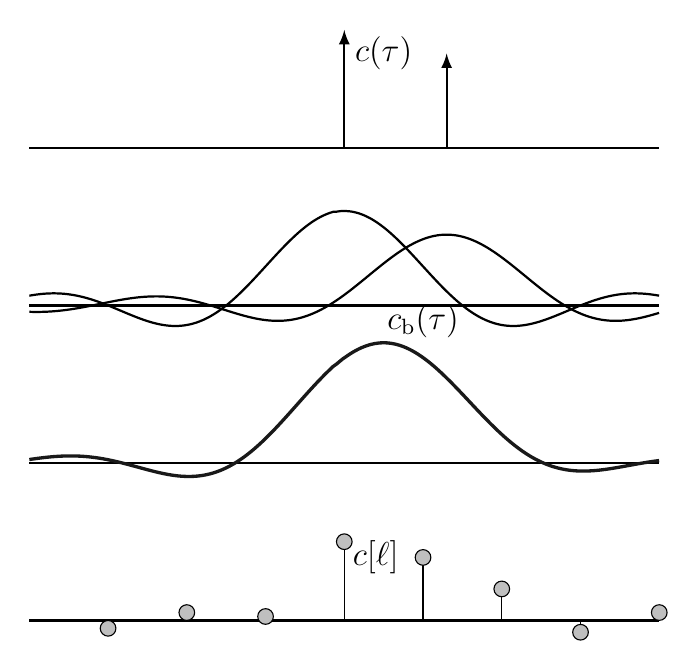
\begin{tikzpicture}[>=latex] % Usa frecce stile LaTeX
    % Definizione stile marker per i campioni
    \tikzset{
        marker/.style={
            circle,
            draw=black,
            thin,
            fill=gray!50,
            inner sep=2pt
        }
    }

    % Parametri per il dominio dell'asse x
    \def\xmin{-4}
    \def\xmax{4}
    % Fattore di scala per l'argomento del seno (controlla la larghezza del lobo)
    \def\k{120} 
    % Fattore di conversione da gradi a radianti per il denominatore
    \def\rad{0.017453} 

    % --- Grafico 1 (In alto): Impulsi c(tau) ---
    \begin{scope}[yshift=6cm]
        % Asse x
        \draw[thick] (\xmin,0) -- (\xmax,0);
        
        % Impulsi (rappresentati come frecce)
        \draw[->, thick] (0,0) -- (0,1.5); % Impulso in 0
        \draw[->, thick] (1.3,0) -- (1.3,1.2); % Impulso in 1.3
        
        % Etichetta
        \node at (0.5, 1.2) {\large $c(\tau)$};
    \end{scope}

    % --- Grafico 2 (Medio-Alto): Componenti separate ---
    \begin{scope}[yshift=4cm]
        % Asse x
        \draw[thick] (\xmin,0) -- (\xmax,0);
        
        % Prima curva (centrata in 0, ampiezza 1.2)
        % Si usa un condizionale per gestire la divisione per zero a x=0
        \draw[thick, smooth, domain=\xmin:\xmax, samples=200] 
            plot (\x, { abs(\x) < 0.001 ? 1.2 : 1.2 * sin(\k*\x) / (\k*\x * \rad) });
            
        % Seconda curva (centrata in 1.3, ampiezza 0.9)
        % Si usa un condizionale per gestire la divisione per zero a x=1.3
        \draw[thick, smooth, domain=\xmin:\xmax, samples=200] 
            plot (\x, { abs(\x-1.3) < 0.001 ? 0.9 : 0.9 * sin(\k*(\x-1.3)) / (\k*(\x-1.3) * \rad) });
    \end{scope}

    % --- Grafico 3 (Medio-Basso): Somma c_b(tau) ---
    \begin{scope}[yshift=2cm]
        % Asse x
        \draw[thick] (\xmin,0) -- (\xmax,0);
        
        % Somma delle due curve precedenti
        % Si sommano le due espressioni condizionali
        \draw[very thick, smooth, color=black!90, domain=\xmin:\xmax, samples=200] 
            plot (\x, { 
                (abs(\x) < 0.001 ? 1.2 : 1.2 * sin(\k*\x) / (\k*\x * \rad)) + 
                (abs(\x-1.3) < 0.001 ? 0.9 : 0.9 * sin(\k*(\x-1.3)) / (\k*(\x-1.3) * \rad)) 
            });
            
        % Etichetta
        \node at (1.0, 1.8) {\large $c_{\text{b}}(\tau)$};
    \end{scope}

    % --- Grafico 4 (In basso): Campionamento c[l] ---
    \begin{scope}[yshift=0cm]
        % Asse x
        \draw[thick] (\xmin,0) -- (\xmax,0);
        
        % Campioni discreti (stem plot)
        % I valori sono scelti per corrispondere visivamente alla curva somma sovrastante
        \draw ( -3, 0) -- (-3, -0.1) node[marker] {};
        \draw ( -2, 0) -- (-2, 0.1) node[marker] {};
        \draw ( -1, 0) -- (-1, 0.05) node[marker] {};
        \draw ( 0, 0) -- ( 0, 1.0) node[marker] {};   % Picco principale
        \draw ( 1, 0) -- ( 1, 0.8) node[marker] {};   % Valore alto dovuto alla sovrapposizione
        \draw ( 2, 0) -- ( 2, 0.4) node[marker] {};   % Coda
        \draw ( 3, 0) -- ( 3, -0.15) node[marker] {}; % Leggermente negativo
        \draw ( 4, 0) -- ( 4, 0.1) node[marker] {};
        
        % Etichetta
        \node at (0.4, 0.8) {\large $c[\ell]$};
    \end{scope}

\end{tikzpicture}
\end{center}

This is a typical example of \textbf{reflection}; for each delta, we'll have a sinc; if we sample this, then we'll have four taps (as can be seen in the last figure).
In this case what happens is that from two taps, in the discrete domain we got 4.

% --- Pagina 3 ---

The amount of taps are increasing; we can only sync with one or the other, thus we're always in trouble.

This is a simple problem: if we only have a tap, we'll have a single tap in the frequency domain.
If we have multiple taps, stuff might become a nightmare!

Sampling is nice, but we can't do this for free.

Let's make some comments on developing a discrete time model:
\begin{itemize}
    \item Noise is still IID and the noise samples are still Gaussian with $\sim \mathcal{N}(0, N_0)$
    \item We can also use root-raised-cosine filter instead of a sinc filter.
    \item If we want to detect a signal, it's much easier to do so if we have a white specter: if the noise goes through certain blocks, though, it will no longer be flat!
\end{itemize}

% Diagramma blocco whitening
\begin{center}
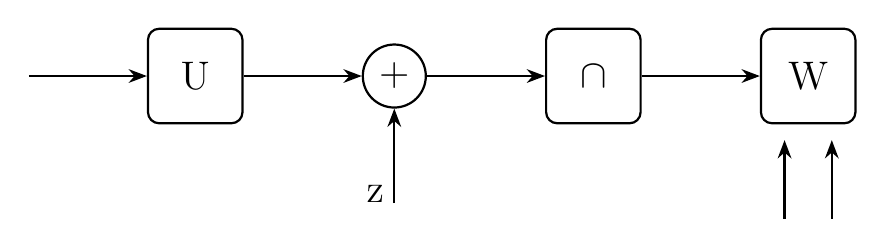
\begin{tikzpicture}[
    >=Stealth, node distance=1.5cm,
    box/.style={draw, rounded corners, minimum size=1.2cm, thick, font=\Large},
    sum/.style={draw, circle, thick, inner sep=0pt, minimum size=0.8cm, font=\Large}
]

% Blocchi principali
\node[box] (U) {U};
\node[sum, right=of U] (sum) {+};
\node[box, right=of sum] (N) {$\cap$};
\node[box, right=of N] (W) {W};

% Frecce di collegamento
\draw[->, thick] ($(U.west)+(-1.5,0)$) -- (U);
\draw[->, thick] (U) -- (sum);
\draw[->, thick] (sum) -- (N);
\draw[->, thick] (N) -- (W);

% Ingresso z al sommatore
\draw[->, thick] ($(sum.south)+(0,-1.2)$) -- (sum) node[pos=0.1, left] {\Large z};

% Frecce sotto W
\draw[->, thick] ($(W.south)+(-0.3,-1.2)$) -- ($(W.south)+(-0.3,-0.2)$);
\draw[->, thick] ($(W.south)+(0.3,-1.2)$) -- ($(W.south)+(0.3,-0.2)$);

\end{tikzpicture}
\end{center}

we can add a \textbf{block which whitens the noise}; this is good since then all the subsequent equalization and such work much better.
Whitening a noise can be much more difficult.

Pulse shaping: if in the frequency domain we have a sinc, this is optimal. This is a sinc tho, which decays slowly in the time domain.
This is why we're using a root-raised-cosine filter: it will have a wider bandwidth but it will be better in the time domain.

Instead of sampling at the Nyquist rate (which allows for perfect recovering), we can say: "what if I sample the signal more frequently? Maybe I can make algorithms which are working better". From the Information theory FOV, Nyquist suffices; but if we have to do with practical issues like non linearities, stuff might be different.
Amplifiers are generally non-constant: there is a certain range in which the amplifier is linear, but there is a certain point at which whichever signal we put at the input of the amplifier, we'll get the exact same output; this is called clipping:

% Grafico Clipping
\begin{center}
\begin{tikzpicture}
    \draw[->] (0,0) -- (2.5,0);
    \draw[->] (0,0) -- (0,1.5);
    \draw (0,0) -- (1,1) -- (2,1); % Rampa poi saturazione
\end{tikzpicture}
\end{center}

\textbf{For synchronization, it helps to have oversampling} (not in the book!); if the Nyquist rate is just in between the right points, it might not sync correctly.

\begin{quote}
    \small \textit{\color{gray} Random stuff about vinils}
\end{quote}
% --- Pagina 1 ---

\section[Transitioning to MIMO]{Transitioning to MIMO (frequency selective and FIR channel expressions; channel normalization)}

We're now going towards MIMO; we have a certain number $N_t$ of transmitting antennas and $N_r$ of receive antennas; those numbers can def be different.

We have at the input the value $\mathbf{x}$ and at the output $\mathbf{y}$ with noise $\mathbf{v}$.

Let's start from the causal and FIR \textbf{frequency flat} channel; we'll have an output of:
\begin{align}
\mathbf{y}[n] = \sqrt{\rho}\mathbf{H}\mathbf{x}[n] + \mathbf{v}[n]. \tag{2.81}
\end{align}

$\mathbf{H}$ is a matrix such that the impulse response between transmit antenna $j$ and receive antenna $i$ will be represented by $\mathbf{H}_{i,j}$.

% Riquadro Blu: Frequency flat
\noindent\fcolorbox{blue}{white}{
    \begin{minipage}{\dimexpr\linewidth-2\fboxsep-2\fboxrule}
        \textcolor{blue}{\textbf{$\diamond$ Frequency flat (also found as frequency-flat)}}
        \vspace{0.5em}
        
        By frequency flat, the book refers to a channel which has just one tap, aka $L=0$.
    \end{minipage}
}

$\mathbf{x}$ is multiplied by $\mathbf{H}$; this means that the \textbf{length of $\mathbf{x}$ is $N_t$}; the length of $\mathbf{y}$ is $N_r$.

% Riquadro Grigio: Skipped
\noindent\fcolorbox{gray}{white}{
    \begin{minipage}{\dimexpr\linewidth-2\fboxsep-2\fboxrule}
        \textcolor{gray}{\textbf{Skipped}}
        \vspace{0.5em}
        
        Professor skipped the beginning of \textbf{section 2.3.1}, which tackles a continuous IO MIMO relation.
    \end{minipage}
}

Just like we saw, we're not certain of having a delta; we might have some other paths!
We'll model this (a \textbf{FIR channel}) just as we did before:
\begin{align}
\mathbf{y}[n] = \sqrt{\rho} \sum_{l=0}^{L-1} \mathbf{H}[l]\mathbf{x}[n-l] + \mathbf{v}[n]. \tag{2.80}
\end{align}
where $[\mathbf{H}[l]]_{i,j}$ represents the response between transmit antenna $j$ and receive antenna $i$.
This means that the \textbf{output vector at time $n$ is also depends on previous symbols}. Each vector is then also weighted by a different matrix, which changes over time.

There is no difference, conceptually, with the scalar case; we only have that we have a matrix instead of a vector.

Before, we had normalized the channel; in this case we sum over all the three indexes; we don't want it to be $1$, but instead we'd like to be $1 \cdot \# \text{ of paths} = \boxed{N_t N_r}$.

We can use the definition of the \textbf{Frobenius norm} in order to impose the normalization; while we could impose the summation to be equal to 1, this would not allow to include channel models with power asymmetry across antennas; for this reason, we have that
\begin{align}
\sum_{l=0}^{L-1} \sum_{i=0}^{N_r-1} \sum_{j=0}^{N_t-1} \mathbb{E}[|H[l]_{i,j}|^2] = N_t N_r. \tag{2.82}
\end{align}

% --- Pagina 2 ---

which can be rewritten more compactly using the definition of Frobenius norm (given in appendix B.5),
\begin{align}
\sum_{l=0}^{L-1} \mathbb{E}[||\mathbf{H}[l]||_F^2] &= \sum_{l=0}^{L-1} \mathbb{E}[\text{tr}(\mathbf{H}[l]\mathbf{H}^H[l])] \tag{2.83} \\
&= \sum_{l=0}^{L-1} \mathbb{E}[\text{tr}(\mathbf{H}^H[l]\mathbf{H}[l])] \tag{2.84} \\
&= N_t N_r. \tag{2.85}
\end{align}
which for the frequency-flat channel simplifies to
\begin{align}
\mathbb{E}[||\mathbf{H}||_F^2] &= \mathbb{E}[\text{tr}(\mathbf{H}\mathbf{H}^H)] \tag{2.86} \\
&= \mathbb{E}[\text{tr}(\mathbf{H}^H\mathbf{H})] \nonumber \\
&= N_t N_r. \nonumber
\end{align}

The Frobenius norm is taking matrix and substituting it with the trace of the matrix multiplied with the complex conjugate of said matrix.

\section{Precoding}

\subsection{Introduction (information theory writing of $x[n]$, matrix $F$; variation of precoded $x$)}

% Diagramma a blocchi colorati (TikZ)
\begin{center}
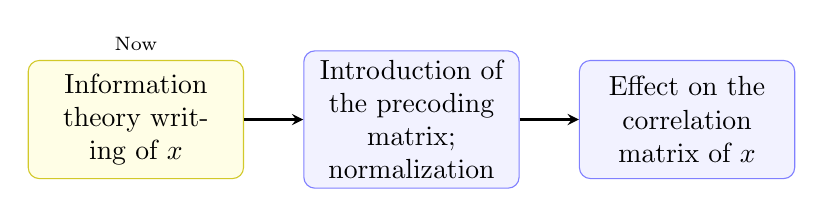
\begin{tikzpicture}[node distance=3.5cm, auto]
    \tikzstyle{yellowblock} = [rectangle, draw=yellow!80!black, fill=yellow!10, text width=2.5cm, text centered, rounded corners, minimum height=1.5cm]
    \tikzstyle{blueblock} = [rectangle, draw=blue!50, fill=blue!5, text width=2.5cm, text centered, rounded corners, minimum height=1.5cm]
    \tikzstyle{arrow} = [thick,->,>=stealth]

    \node [yellowblock] (start) {Information theory writing of $x$};
    \node [coordinate, above of=start, node distance=1cm] (nowlabel) {}; 
    \node [above] at (start.north) {\scriptsize Now};
    
    \node [blueblock, right of=start] (middle) {Introduction of the precoding matrix; normalization};
    \node [blueblock, right of=middle] (end) {Effect on the correlation matrix of $x$};

    \draw [arrow] (start) -- (middle);
    \draw [arrow] (middle) -- (end);
\end{tikzpicture}
\end{center}

We have the precoding; we'll start with SISO signals. We'll decompose it in an IT (Information Theory) friendly way:
\begin{align*}
x[n] = \sqrt{E_s P[n]} s[n].
\end{align*}
where:
\begin{itemize}
    \item $E_s$ is the average symbol energy
    \item $P[n]$ is the power allocation at a certain given time
    \item $s[n]$ are unit-variance symbols (PSK, QAM, Gaussian)
\end{itemize}

% Riquadro Viola 1
\noindent\fcolorbox{violet}{white}{
    \begin{minipage}{\dimexpr\linewidth-2\fboxsep-2\fboxrule}
        \textcolor{violet}{\textbf{Hello, new writing of $x[n]$! Will you stick around?}}
        \vspace{0.5em}
        
        Yup. This writing will be reused in chapter 4, when linking OFDM and vector coding (and also when finding the SNR for both).
    \end{minipage}
}
\vspace{1em}

% Riquadro Viola 2
\noindent\fcolorbox{violet}{white}{
    \begin{minipage}{\dimexpr\linewidth-2\fboxsep-2\fboxrule}
        \textcolor{violet}{\textbf{About units...}}
        \vspace{0.5em}
        
        From what I gather, if we admit that energy is in $W \cdot s$ and power in $W$, if $x$ is in units of $V$, then $s$ must have a unit of $V/\sqrt{J}$.
    \end{minipage}
}

% --- Pagina 3 ---


Sending info using a Gaussian: a \textbf{Gaussian} is the base we use for the other ways to send signals; we use it as a \textbf{bound} for what we can do.
If we don't reach the performance of the Gaussian, there is a reason for that.

When we're going from 16 to 64 QAM, we're just making the constellation more dense.

% Testo con sfondo verde chiaro
\noindent\colorbox{green!10}{
    \begin{minipage}{\dimexpr\linewidth-2\fboxsep}
        $P[n]$ is the power allocation for each signal; about it: \\
        In our phone we have an algorithm called the \textit{power control algorithm}; when we go away from an antenna, we need to raise the power used to transmit; if we're close, we need to have a forward signal! \\
        What is practically done is that we measure the signal from the base station and we'll know how strong our signal should be. \\
        We'll then change the signal when we go farther from a station.
    \end{minipage}
}

% Diagramma ripetuto con enfasi (TikZ)
\begin{center}
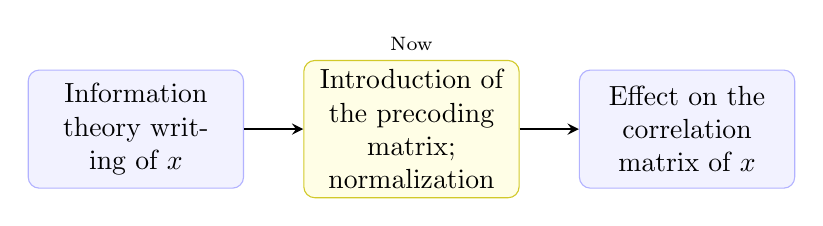
\begin{tikzpicture}[node distance=3.5cm, auto]
    \tikzstyle{block} = [rectangle, draw=blue!30, fill=blue!5, text width=2.5cm, text centered, rounded corners, minimum height=1.5cm]
    \tikzstyle{focus} = [rectangle, draw=yellow!80!black, fill=yellow!10, text width=2.5cm, text centered, rounded corners, minimum height=1.5cm]
    \tikzstyle{arrow} = [thick,->,>=stealth]

    \node [block] (start) {Information theory writing of $x$};
    \node [focus, right of=start] (middle) {Introduction of the precoding matrix; normalization};
    \node [above] at (middle.north) {\scriptsize Now};
    \node [block, right of=middle] (end) {Effect on the correlation matrix of $x$};

    \draw [arrow] (start) -- (middle);
    \draw [arrow] (middle) -- (end);
\end{tikzpicture}
\end{center}

With MIMO we do \textit{transmit precoding}: we suppose we have $N_s \leq N_t$: the number of transmit symbols ($N_s$) is at most equal to the number of transmit antennas ($N_t$).
If we're not using an antenna, we can think about what to do with it. If we have 5 symbols but just an antenna, we won't be able to transmit that symbol. \textbf{Our vector of symbols can only be transmitted if $N_s \leq N_t$}.
In the MIMO we can do more than deciding how much power we should use.

% Disegno "handwritten" del precoder matrix -> antennas
\begin{center}
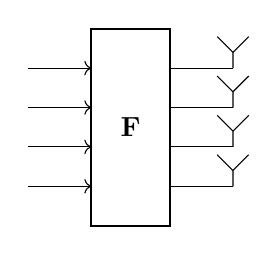
\begin{tikzpicture}
    % Matrix block
    \draw[thick] (0,0) rectangle (1,2.5);
    \node at (0.5, 1.25) {$\mathbf{F}$}; % Matrice precoding
    
    % Input lines (sinistra)
    \foreach \y in {0.5, 1.0, 1.5, 2.0} {
        \draw[<-] (0,\y) -- (-0.8, \y);
    }
    
    % Output lines + Antennas (destra)
    \foreach \y in {0.5, 1.0, 1.5, 2.0} {
        \draw (1,\y) -- (1.8, \y);
        % Antenna drawing
        \draw (1.8, \y) -- (1.8, \y+0.2) -- (1.6, \y+0.4);
        \draw (1.8, \y+0.2) -- (2.0, \y+0.4);
    }
\end{tikzpicture}
\end{center}

we might decide to use a matrix to mix those symbols; it's a degree of freedom which might prove very useful: why not use it?

For any running symbol, we multiply it with a matrix $\mathbf{F}[n]$ (which can vary with $n$!!):
\begin{align}
\mathbf{x}[n] = \sqrt{\frac{E_s}{N_t}} \mathbf{F}[n]\mathbf{s}[n]. \tag{2.96}
\end{align}
% --- Pagina 1 (Continuazione) ---

where:
\begin{itemize}
    \item The $s[n]$ symbols are \textcolor{green!60!black}{\textbf{IID}}.
    \item $E_s$ is the average energy per symbol (more about this later).
    \item $F[n]$ is the precoder matrix; as we'll see, it's normalized in order to respect specific relations. It will have a dimension of $N_t \times N_s$.
\end{itemize}

We have a restriction on $F[n]$ which uses the \textbf{Frobenius norm}; it grants that the antenna is not amplifying the signal:
\begin{align}
\frac{1}{N} \sum_{n=0}^{N-1} ||\mathbf{F}[n]||_F^2 = \frac{1}{N} \sum_{n=0}^{N-1} \text{tr}(\mathbf{F}[n]\mathbf{F}^H[n]) = N_t. \tag{2.97}
\end{align}

Later, we'll need the transmit covariance.
$s[n]$ are IID codewords, which means that $\mathbb{E}[\mathbf{s}[n]\mathbf{s}^*[n]] = \mathbf{I}$ (this follows from the fact that independence implies uncorrelation and that these vectors are 0-mean; the main diagonal will have the variance of each signal, which is 1), with dimensions $N_s \times N_s$.

% Box verdino chiaro
\noindent\colorbox{teal!10}{
    \begin{minipage}{\dimexpr\linewidth-2\fboxsep}
        We're always transmitting 0-mean and 1-variance signals.
    \end{minipage}
}

% Diagramma a blocchi (Focus sul terzo blocco)
\begin{center}
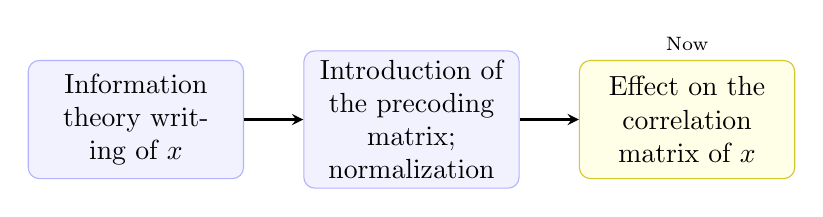
\begin{tikzpicture}[node distance=3.5cm, auto]
    \tikzstyle{block} = [rectangle, draw=blue!30, fill=blue!5, text width=2.5cm, text centered, rounded corners, minimum height=1.5cm]
    \tikzstyle{focus} = [rectangle, draw=yellow!80!black, fill=yellow!10, text width=2.5cm, text centered, rounded corners, minimum height=1.5cm]
    \tikzstyle{arrow} = [thick,->,>=stealth]

    \node [block] (start) {Information theory writing of $x$};
    \node [block, right of=start] (middle) {Introduction of the precoding matrix; normalization};
    \node [focus, right of=middle] (end) {Effect on the correlation matrix of $x$};
    \node [above] at (end.north) {\scriptsize Now};

    \draw [arrow] (start) -- (middle);
    \draw [arrow] (middle) -- (end);
\end{tikzpicture}
\end{center}

If we take into account $x[n]$, which has multiplication with the matrix, the covariance will be given by $\mathbf{R_x}$.
In order to find its value, we'll apply the fact that $(\mathbf{F}\mathbf{s})^* = \mathbf{s}^*\mathbf{F}^*$.
We'll thus have
\begin{align}
\mathbf{R_x} &= \frac{E_s}{N_t} \mathbb{E}[\mathbf{F}\mathbf{s}\mathbf{s}^*\mathbf{F}^*] \nonumber \\
&= \frac{E_s}{N_t} \mathbf{F} \mathbb{E}[\mathbf{s}\mathbf{s}^*] \mathbf{F}^* \nonumber \\
&\overset{(*)}{=} \frac{E_s}{N_t} \mathbf{F} \mathbf{F}^*. \nonumber
\end{align}

re-introducing the time dependent notation, we have (for ID $\mathbf{s}$)
\begin{align}
\mathbf{R_x}[n] = \frac{E_s}{N_t} \mathbf{F}[n]\mathbf{F}^H[n]. \tag{2.101}
\end{align}

% Riquadro Viola: Comparison
\noindent\fcolorbox{violet}{white}{
    \begin{minipage}{\dimexpr\linewidth-2\fboxsep-2\fboxrule}
        \textcolor{violet}{\textbf{\faIcon{book} Comparison with normal case}}
        \vspace{0.5em}
        
        If we were to set $\mathbf{F}[n] = \mathbf{I}$, we'd find that the non-precoded matrix of $x$ is
        \[ \frac{E_s}{N_t}\mathbf{I}. \]
    \end{minipage}
}

We have a source of symbols, we pass them through a serial to parallel and then we go through the antennas; usually, we use a code

% --- Pagina 2 ---


% Disegno Serial to Parallel (S/P) -> Antenne
\begin{center}
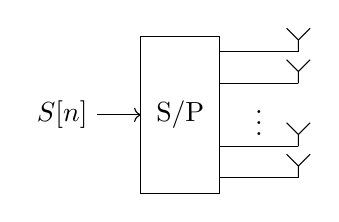
\begin{tikzpicture}
    \node (s) at (-1, 0) {$S[n]$};
    \draw[->] (s) -- (0,0);
    
    % Box S/P
    \draw (0,-1) rectangle (1,1);
    \node at (0.5,0) {S/P};
    
    % Uscite verso antenne
    \foreach \y in {0.8, 0.4, -0.4, -0.8} {
        \draw (1,\y) -- (2,\y);
        \draw (2,\y) -- (2,\y+0.15) -- (1.85, \y+0.3);
        \draw (2,\y+0.15) -- (2.15, \y+0.3);
    }
    \node at (1.5, 0) {$\vdots$};
\end{tikzpicture}
\end{center}

What we generally do is actually code after the series/parallel transition!

% Disegno Coding -> S/P -> PREC -> Antenne
\begin{center}
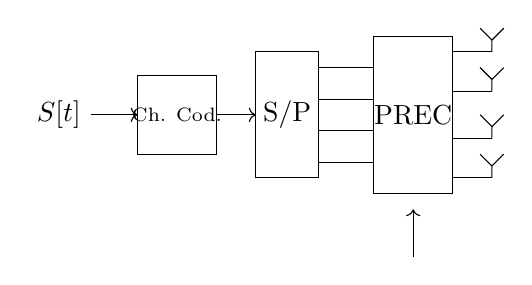
\begin{tikzpicture}
    \node (s) at (-2.5, 0) {$S[t]$};
    
    % Block Code
    \draw (-1.5,-0.5) rectangle (-0.5,0.5);
    \node at (-1,0) {\scriptsize Ch. Cod.};
    \draw[->] (s) -- (-1.5,0);
    \draw[->] (-0.5,0) -- (0,0);
    
    % Box S/P
    \draw (0,-0.8) rectangle (0.8,0.8);
    \node at (0.4,0) {S/P};
    
    % Box PREC
    \draw (1.5,-1) rectangle (2.5,1);
    \node at (2,0) {PREC};
    
    % Connections S/P -> PREC
    \foreach \y in {0.6, 0.2, -0.2, -0.6} {
        \draw (0.8,\y) -- (1.5,\y);
    }
    
    % Outputs PREC -> Antenne
    \foreach \y in {0.8, 0.3, -0.3, -0.8} {
        \draw (2.5,\y) -- (3,\y);
        \draw (3,\y) -- (3,\y+0.15) -- (2.85, \y+0.3);
        \draw (3,\y+0.15) -- (3.15, \y+0.3);
    }
    
    % Freccia indicativa sotto PREC
    \draw[<-] (2,-1.2) -- (2,-1.8);
\end{tikzpicture}
\end{center}

\section{Recap of singular value decomposition}

Let's revisit the concept of singular value decomposition!

% Riquadro verde chiaro
\noindent\colorbox{teal!10}{
    \begin{minipage}{\dimexpr\linewidth-2\fboxsep}
        This is heavily used in machine learning and such
    \end{minipage}
}

We have a certain matrix $\mathbf{A}$ of dimensions $N \times M$; we can always decompose it as
\[ \mathbf{A} = \mathbf{U} \mathbf{\Sigma} \mathbf{V}^*, \]
where:
\begin{itemize}
    \item $\mathbf{U}$ is unitary $N \times N$.
    \item $\mathbf{V}^*$ is unitary $M \times M$.
    \item $\mathbf{\Sigma}$ is $N \times M$ with non negative entries on its diagonal ordered from largest to smallest.
\end{itemize}
The entries of said matrix \textbf{are the singular values of the original matrix, aka the square root of the eigenvalues of $\mathbf{A}$}.

The $\mathbf{\Sigma}$ matrix is generally like

% Disegno schizzato della matrice Sigma
\begin{center}
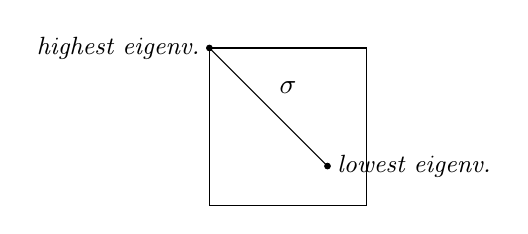
\begin{tikzpicture}
    \draw (0,0) rectangle (2,2); % Contorno matrice
    \draw (0,2) -- (1.5, 0.5); % Diagonale parziale
    \filldraw (0,2) circle (1pt) node[anchor=east] {\small \textit{highest eigenv.}};
    \filldraw (1.5,0.5) circle (1pt) node[anchor=west] {\small \textit{lowest eigenv.}};
    \node at (1,1.5) {$\sigma$};
\end{tikzpicture}
\end{center}

% --- Pagina 3 ---


If we choose $\mathbf{u}_j$, a column of $\mathbf{V}$ and $\mathbf{u}_j$, a column of $\mathbf{U}$, we'll have
\begin{align*}
\mathbf{A}\mathbf{v}_j &= \sigma_j \mathbf{u}_j \\
\mathbf{A}^*\mathbf{u}_j &= \sigma_j \mathbf{v}_j
\end{align*}
where $\sigma_j$ is the $j$-th element on the diagonal of $\mathbf{\Sigma}$.

We just need to remember the dimensions in order to have this work correctly.

% Riquadro Blu: Property of unitary matrices
\noindent\fcolorbox{blue}{white}{
    \begin{minipage}{\dimexpr\linewidth-2\fboxsep-2\fboxrule}
        \textcolor{blue}{\textbf{\faIcon{pen} Property of unitary matrices}}
        \vspace{0.5em}
        
        For a unitary matrix, we have that
        \[ \mathbf{U}^{-1} = \mathbf{U}^*. \]
        This is why unitary matrices are very useful.
    \end{minipage}
}

$\mathbf{U}$ is very easy to invert and same goes for $\mathbf{V}$. Then we might say: it will be easy to invert $\mathbf{A}$.

$\mathbf{A}$ will also have the following properties:

% Tabella B.1
\begin{center}
\begin{tabular}{lll}
    \toprule
    \multicolumn{3}{l}{\textbf{Table B.1} Bases for the column, row, and null spaces of an $N \times M$ matrix $\mathbf{A} = \mathbf{U \Sigma V}^*$} \\
    \midrule
    \textbf{Subspace} & \textbf{Dimension} & \textbf{Basis} \\
    \midrule
    Column space of $\mathbf{A}$ & $r = \text{rank}(\mathbf{A})$ & First $r$ columns of $\mathbf{U}$ \\
    Row space of $\mathbf{A}$ & $r$ & First $r$ columns of $\mathbf{V}$ \\
    Null space of $\mathbf{A}^T$ & $(N-r)$ & Last $(N-r)$ columns of $\mathbf{U}$ \\
    Null space of $\mathbf{A}$ & $(M-r)$ & Last $(M-r)$ columns of $\mathbf{V}$ \\
    \bottomrule
\end{tabular}
\end{center}

\subsection*{About the number of streams}

If we have 1 transmitter and 1 receiver, we know many things; but we didn't consider a channel which is dispersive and generates ISI; how do we deal with ISI?? This is handled in \textcolor{green}{section 2.5} of the book.

Let's suppose, at least for now, that we have no ISI; the Shannon bound tells us that we have a maximum amount of bits per symbol per hertz which we can put through the channel.

People said: we want to transmit even more!! In order to do so, we increase the number of transmitter and receiver antennas.
Let's say we have 3 transmitters and 5 receivers; the interactions between all of these won't be described by a vector anymore, but rather by a matrix.
We'll see that we have \textbf{a number of independent streams which is}
\[ \# \text{streams} \leq \min \{N_t, N_r\}; \]
we use MIMO since we want to be able to transmit even more than what would have been possible while respecting the Shannon bound.
It's useless to have 1 transmitter and many receivers: we'd be able to only have 1 stream.
% --- Pagina 1 ---

It's difficult to have many antennas in the phone, much more than it is to have many in our station.

Before looking at this, we want to understand if this works at all, though! We first need to know the theory and that this is possible and only then will we be able to use this.

\section[Applying precoding]{Applying precoding: decomposing F and explaining the various parts of its new form}

Let's apply what we've learned to the model
\begin{align}
\mathbf{x}[n] = \sqrt{\frac{E_s}{N_t}} \mathbf{F}[n]\mathbf{s}[n], \tag{2.98}
\end{align}
we know we have $\mathbf{s}[n]$ at the input and let's suppose that $\mathbf{F} = \mathbf{I}$: we go directly in the antennas. If we do this, all the antennas transmit all like a circle (this depends on how they're built), as it comes.
If we then have $\mathbf{F} \neq \mathbf{I}$, we can get each antenna to point to a specific user; this allows us to maximize the gain we have from the transmit antenna.

\begin{figure}[h]
    %immagine centrata
    \centering
    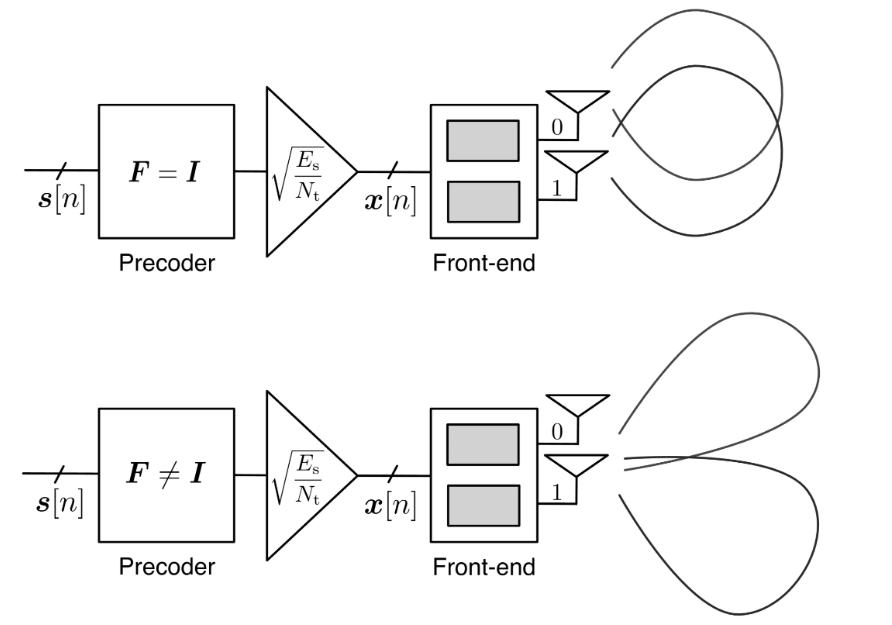
\includegraphics[width=0.6\textwidth]{Pictures/precoder types.png}

\end{figure}

What we want to do is to multiply our symbols with a matrix and do something. What can we achieve?
In order to better understand this, we can use \textcolor{green!60!black}{singular value decomposition} to decompose $\mathbf{F}$ as:
\begin{align}
\mathbf{F}[n] = \mathbf{U}_F[n] \mathbf{\Sigma}_F[n] \mathbf{V}_F^H[n], \tag{2.100}
\end{align}
where:
\begin{itemize}
    \item $\mathbf{V}$ is the \textbf{mixing matrix}, which is a $N_s \times N_s$ unitary matrix
    \item $\mathbf{\Sigma}$ is the \textbf{power allocation matrix} and is $N_t \times N_s$ (more about this later)
    \item $\mathbf{U}$ is the \textbf{beam steering matrix}, which is a $N_t \times N_t$ unitary matrix
\end{itemize}

If we had only
\[ \mathbf{V}_F^* \mathbf{s}, \]
we'd get $N_t$ symbols; this mixes the various signals towards the various antennas:

% --- Pagina 2 ---


% Disegno Mixing (Linee incrociate)
\begin{center}
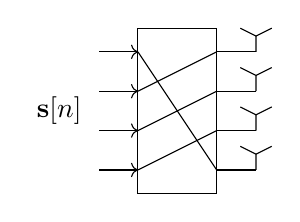
\begin{tikzpicture}
    % Input symbols
    \foreach \y in {2, 1.5, 1, 0.5} {
        \draw[<-] (0,\y) -- (-0.5, \y);
    }
    \node at (-1, 1.25) {$\mathbf{s}[n]$};

    % Mixing block outline
    \draw (0,0.2) rectangle (1, 2.3);
    
    % Lines connecting Inputs to Outputs (Randomized mixing look)
    \draw (0,2) -- (1, 0.5);
    \draw (0,1.5) -- (1, 2);
    \draw (0,1) -- (1, 1.5);
    \draw (0,0.5) -- (1, 1);
    
    % Output antennas
    \foreach \y in {2, 1.5, 1, 0.5} {
        \draw (1,\y) -- (1.5, \y);
        \draw (1.5, \y) -- (1.5, \y+0.2) -- (1.3, \y+0.3); % Antenna parts
        \draw (1.5, \y+0.2) -- (1.7, \y+0.3);
    }
\end{tikzpicture}
\end{center}

By only doing this we'd create confusion; this is why we also have a power allocation matrix: it has a diagonal which expresses how much power we'll give to each antenna.
It will have a shape like
\begin{align}
\mathbf{\Sigma}_F[n] = \begin{bmatrix} \mathbf{P}^{\frac{1}{2}} \\ \mathbf{0} \end{bmatrix} \tag{2.101}
\end{align}
where $\mathbf{P}$ is a $N_s \times N_s$ matrix which will be defined below.

What's really important is $\mathbf{U}_F$, which allows us to \textbf{steer the signal}.

This had been discovered a long time ago! If we have a radar and we transmit with a phase shift on one antenna:

% Disegno Phased Array
\begin{center}
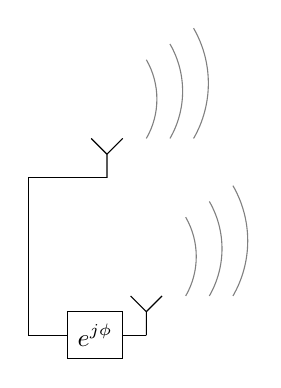
\begin{tikzpicture}
    % Antenne e linea di alimentazione
    \draw (0,0) -- (0, -2); % Cavo principale
    \draw (0,0) -- (1,0); % Top branch
    \draw (0,-2) -- (0.5, -2); % Bottom branch
    
    % Phase shifter box
    \draw (0.5, -2.3) rectangle (1.2, -1.7);
    \node at (0.85, -2) {\small $e^{j\phi}$};
    \draw (1.2, -2) -- (1.5, -2);

    % Antenne
    \foreach \point in {(1,0), (1.5,-2)} {
        \draw \point -- ++(0, 0.3) -- ++(-0.2, 0.2);
        \draw \point ++(0, 0.3) -- ++(0.2, 0.2);
    }

    % Onde radio (simboliche)
    \draw [gray] (1.5, 0.5) arc (-30:30:1);
    \draw [gray] (1.8, 0.5) arc (-30:30:1.2);
    \draw [gray] (2.1, 0.5) arc (-30:30:1.4);

    \draw [gray] (2.0, -1.5) arc (-30:30:1);
    \draw [gray] (2.3, -1.5) arc (-30:30:1.2);
    \draw [gray] (2.6, -1.5) arc (-30:30:1.4);

\end{tikzpicture}
\end{center}

In a certain direction we'll have a specific $\phi$; if $\phi = \pi$, we're not transmitting anything.
If we look at another direction, we can tilt an antenna electronically to transmit over a certain direction.

% --- Pagina 3 ---

This is used by radars, even though radars transmit an impulse and want to get stuff back. In order to understand where the signal is coming from they use multiple antennas and they use something like a steering matrix.
If we take the nose of an airplane, the whole nose of an airplane has a radar in it.

% Box verdino
\noindent\colorbox{teal!10}{
    \begin{minipage}{\dimexpr\linewidth-2\fboxsep}
        It's nothing new in this sense!
    \end{minipage}
}

So now we can have different directions from an array of antennas.
By using appropriate matrices, we can make spatial streams.

Our tools for designing are $\mathbf{U}_F$ and the amount of power we put in each antenna (the sum of the power cannot be more than $N_t$), expressed by the matrix
\[ \mathbf{P} = \text{diag}(P_1, \dots, P_{N_s-1}) \]
such that $\sum_{i=0}^{N_s-1} P_i = N_t$.

The notation $P_j$ is especially interesting since the $j$th mixed signal (aka $[\mathbf{V}_F^H \mathbf{s}[n]]_j$) will have a power of $\frac{E_s}{N_t}P_j$ allocated to it, where the $E_s/N_t$ term comes from our definition in (2.98).

The $j$th amplified signal will be launched from all transmit antennas and will be weighted with the coefficients in the $j$th column of $\mathbf{U}_F[n]$.

If we were to choose a silly (aka useless) setup, we might have both $\mathbf{U}_F, \mathbf{V}_F$ be identity matrices and $\mathbf{P} = \frac{N_t}{N_s}\mathbf{I}$, which entails
\begin{align}
\mathbf{F}[n] = \sqrt{\frac{N_t}{N_s}} \begin{bmatrix} \mathbf{I}_{N_s} \\ \mathbf{0} \end{bmatrix}. \tag{2.102}
\end{align}

With such trivial precoder, each of $N_s$ antennas directly radiates one of the data streams within $\mathbf{s}[n]$ while the remaining $N_t - N_s$ antennas are silent; the transmit signals are independent. If this is the case, the transmission is said to be \textit{isotropic} from a precoding pov or even \textit{unprecoded}.

\noindent\fcolorbox{violet}{white}{
    \begin{minipage}{\dimexpr\linewidth-2\fboxsep-2\fboxrule}
        \textcolor{violet}{\textbf{\faIcon{list-ul} Example 2.10}} \\
        Let $N_t = N_s = 2$ and suppose that the two signals within $s[n]$ are QPSK-distributed.
        Examine the structure of the transmit signal $x[n]$ produced by a time-invariant precoder.

        \vspace{0.5em}
        \textbf{Solution} \\
        Dropping the dependence on $n$, let $\mathbf{P} = \text{diag}(P_1, P_2)$ and
        \begin{align}
        \mathbf{U}_F = \begin{bmatrix} U_{00} & U_{01} \\ U_{10} & U_{11} \end{bmatrix}, \qquad
        \mathbf{V}_F = \begin{bmatrix} V_{00} & V_{01} \\ V_{10} & V_{11} \end{bmatrix}. \tag{2.103}
        \end{align}
        The application of the mixing matrix to $\mathbf{s}$ yields the mixed signal vector
        \begin{align}
        \mathbf{V}_F^* \mathbf{s} = \begin{bmatrix} V_{00}^* (\mathbf{s})_0 + V_{10}^* (\mathbf{s})_1 \\ V_{01}^* (\mathbf{s})_0 + V_{11}^* (\mathbf{s})_1 \end{bmatrix} \tag{2.104}
        \end{align}
        whose unit-variance entries conform to 16-ary distributions, in general distinct. Then, after power allocation,
        \begin{align}
        \sqrt{\frac{E_s}{2}} \mathbf{P}^{1/2} \mathbf{V}_F^* \mathbf{s} = \begin{bmatrix} \sqrt{\frac{E_s P_1}{2}} (V_{00}^* (\mathbf{s})_0 + V_{10}^* (\mathbf{s})_1) \\ \sqrt{\frac{E_s P_2}{2}} (V_{01}^* (\mathbf{s})_0 + V_{11}^* (\mathbf{s})_1) \end{bmatrix}. \tag{2.105}
        \end{align}
        The top signal is launched from the two antennas, weighted by $U_{00}$ and $U_{10}$, while the bottom signal is launched weighted by $U_{01}$ and $U_{11}$. If $\mathbf{F} = \mathbf{I}$, then each signal is radiated from only one antenna. Conversely, if $\mathbf{F} \neq \mathbf{I}$, each signal is transmitted from both antennas and steered in a certain direction. Both possibilities are illustrated in Fig. 2.11.

        \vspace{0.5em}
        \textbf{Comments:}
        \begin{itemize}
            \item The $*$ operator on matrix also implies transposition
            \item A unitary matrix is just rotating the vector: it won't change its magnitude
            \item If $\mathbf{F} = \mathbf{I}$, each signal is radiated by one antenna
            \item If $\mathbf{F} \neq \mathbf{I}$, both signals are transmitted by both antennas and we can steer the antennas.
        \end{itemize}
    \end{minipage}
}

\section[Signal power constraints]{Signal power constraints}

Which power constraint will we enforce? We might have average energy per block or per symbol or even per antenna:

\begin{itemize}
    \item[\textcolor{red}{$\blacksquare$}] \textbf{Per-block} $\frac{1}{N} \sum_{n} ||\mathbf{x}[n]||^2 \le P$, or equivalently $\frac{1}{N} \sum_{n} \text{tr}(\mathbf{R_x}[n]) = P_t$.
    
    {\small $\rightarrow$ Then the precoder $\frac{1}{N} \sum_{n} ||\mathbf{F}[n]||^2_F = N_t$}

    \item[\textcolor{red}{$\blacksquare$}] \textbf{Per-symbol} $\mathbb{E}[||\mathbf{x}[n]||^2] = E_s$ or $\text{tr}(\mathbf{R_x}[n]) = E_s$
    
    {\small $\rightarrow$ Then the precoder satisfies $\text{tr}(\mathbf{F}[n]\mathbf{F}^H[n]) = \text{tr}(\mathbf{P}[n]) = N_t$}
    
    \item[\textcolor{red}{$\blacksquare$}] \textbf{Per-antenna} $(\mathbf{R_x})_{ii} = \frac{E_s}{N_t}$, which means that
    
    {\small $||\mathbf{F}[n]||^2_{i,:} = 1 \text{ for } i = 0, \dots, N_t-1$}
\end{itemize}

% --- Pagina 2 ---


We might even be super strict and say \textit{every symbol should have the same energy}, or more relaxed and say: on average a block should have a certain amount of energy.
What we have depends on our situation.

% Riquadro Examples
\noindent\fcolorbox{violet}{white}{
    \begin{minipage}{\dimexpr\linewidth-2\fboxsep-2\fboxrule}
        \textcolor{violet}{\textbf{\faIcon{list-ul} Examples}}
        \vspace{0.5em}
        
        Regulation says that if we put a sphere around the top of the antenna; the power of the outgoing em field should be below a certain value. If we have that power, we'll need to share it between antennas.
        
        If we have DAS (Distributed Antenna System), which is now used in tunnels, we can put the same power on the various antennas.
    \end{minipage}
}

The constraint depends on the practical situation which we have.

\section[Vectorizing the channel]{Vectorizing the channel: MIMO multipath channel (specifically, stacked notation absorbing convolution, time dependency and MIMO) for receiver $i$ and for the whole system}

We were looking at how to vectorize the channel; this paragraph, specifically, investigates how to reach for MIMO a result similar to the (2.74) we reached for SISO.
We also include previous values of the signal since the channel has memory.
This is like convolution, but in the time domain.

Now, instead of having SISO systems, we can jump to the MIMO case. In summary, instead of having scalars in the matrix $H$, in the MIMO system we'll have matrices.

% Diagramma MIMO H(0)
\begin{figure}[h]
    \centering
    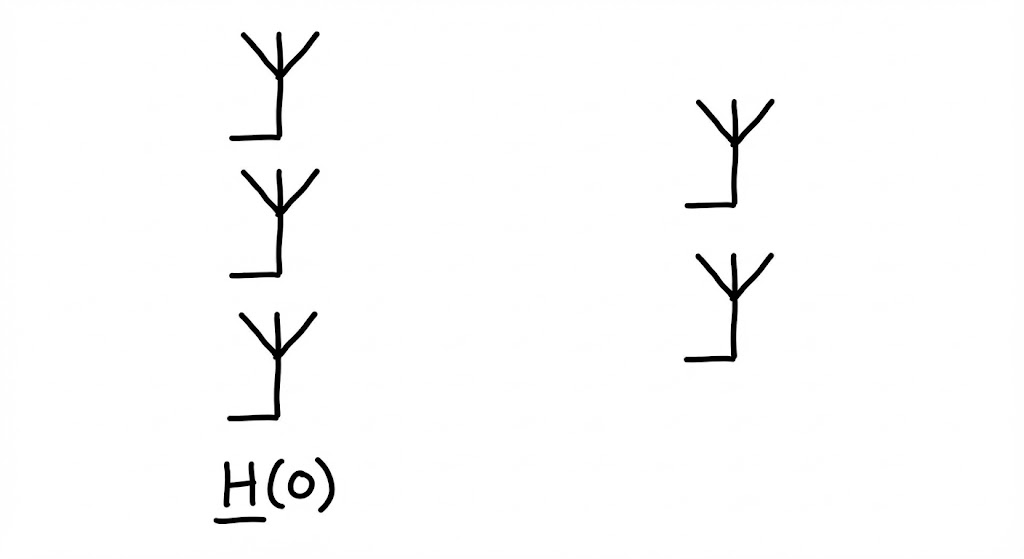
\includegraphics[width=0.6\textwidth]{Pictures/antennas.png}
\end{figure}

$H(0)$ tells how the signal gets from one part to the other.
In the SISO case we had $h[k], k=0, \dots, L$: we had $L$ paths since we weren't in a flat channel.
We won't stop at considering only the matrix corresponding to $h[0]$; we'll also look at the matrix for the system's memory.

If we then consider the receiver antenna $i$, we'll have that the received signal will be the sum of all the values:
\begin{align}
y_i^{(r)} = \sqrt{\rho} \sum_{j=0}^{N_t-1} [\mathbf{H}]_{i,j} \mathbf{x}_j^{(N+L)} + \mathbf{v}_i^{(r)}. \tag{2.89}
\end{align}
where $\mathbf{H}$ is a matrix of matrices and $N+L$ is there since we have $L$ delays.
The output does not only depend on one input vector, but it's still a vector of dimension $N+L$ depending on the input of each transmit antenna ($x_j^{(N+L)}$).

% Riquadro Viola: What are those subscripts
\noindent\fcolorbox{violet}{white}{
    \begin{minipage}{\dimexpr\linewidth-2\fboxsep-2\fboxrule}
        \textcolor{violet}{\textbf{\faIcon{book} What are those $N, N+L$ subscripts?}}
        \vspace{0.5em}
        
        Those subscripts represent the dimensions of vectors and matrices.
        Just as an example, $\mathbf{x}$ is a $(N+L) \times 1$ vector and $\mathbf{H}$ is a $N \times (N+L)$ matrix.
        
        Specifically, then, each vector contains the time information for signals for $n=0, \dots, N-1$, with the relation $\mathbf{H}\mathbf{x}$ representing the convolution operation.
    \end{minipage}
}

We're considering the antenna $i$:

% Diagramma SISO link j -> i
\begin{center}
\begin{tikzpicture}
    % Antenna j
    \draw (0,1) -- (0,1.3) -- (-0.2, 1.5);
    \draw (0,1.3) -- (0.2, 1.5);
    \node[left] at (-0.2, 1.3) {$j$};
    
    % Antenna i
    \draw (4,1) -- (4,1.3) -- (3.8, 1.5);
    \draw (4,1.3) -- (4.2, 1.5);
    \node[right] at (4.2, 1.3) {$i$};
    
    % Freccia collegamento
    \draw[->] (0.5, 1.2) -- (3.5, 0.8);
    
    % Altre antenne sfumate (contesto)
    \node at (0, 0.5) {$\vdots$};
    \node at (4, 0.5) {$\vdots$};
    
    \node at (2, -0.5) {\Large \textit{\color{gray} SISO!}};
\end{tikzpicture}
\end{center}

We have many antennas transmitting to $i$; we need to sum over all the transmitting antennas and over all the vectors transmitted at the $j$-th antenna.
The jump we're doing with this new equation is given by the fact that we have many transmission antennas!
$y$ will have a dimension of $N_r N$! We're putting the various vectors one on top of the other:
% --- Pagina 1 ---

\begin{align*}
\bar{\boldsymbol{y}}_{N_r N} = \begin{bmatrix} \bar{\boldsymbol{y}}_N^{(0)} \\ \vdots \\ \bar{\boldsymbol{y}}_N^{(N_r-1)} \end{bmatrix}.
\end{align*}

\vspace{1em}

\begin{align*}
\bar{\boldsymbol{x}}_{N_t(N+L)} = \begin{bmatrix} \bar{\boldsymbol{x}}_{N+L}^{(0)} \\ \vdots \\ \bar{\boldsymbol{x}}_{N+L}^{(N_t-1)} \end{bmatrix}.
\end{align*}

Before we had $N, N+L$ on the matrix; now we have $N_r N, N_t(N+L)$.
The input vector is $N_t(N+L)$: we're stacking the vectors of the input antennas.

All the matrices in H are $N, N+L$ matrices:
\begin{align*}
\begin{bmatrix}
\bar{\boldsymbol{H}}_{N,N+L}^{(0,0)} & \bar{\boldsymbol{H}}_{N,N+L}^{(0,1)} & \cdots & \bar{\boldsymbol{H}}_{N,N+L}^{(0, N_t-1)} \\
\bar{\boldsymbol{H}}_{N,N+L}^{(1,0)} & \bar{\boldsymbol{H}}_{N,N+L}^{(1,1)} & \cdots & \bar{\boldsymbol{H}}_{N,N+L}^{(1, N_t-1)} \\
\vdots & \vdots & \ddots & \vdots \\
\bar{\boldsymbol{H}}_{N,N+L}^{(N_r-1,0)} & \bar{\boldsymbol{H}}_{N,N+L}^{(N_r-1,1)} & \cdots & \bar{\boldsymbol{H}}_{N,N+L}^{(N_r-1, N_t-1)}
\end{bmatrix}
\end{align*}

Each of the matrices is like a SISO matrix; we're considering how the information transmitted from antenna $j$ is arriving at antenna $i$.

In summary, we can express the output of the MIMO system as
\begin{align}
\bar{\boldsymbol{y}}_{N_r N} = \sqrt{G} \bar{\boldsymbol{H}}_{N_r N, N_t(N+L)} \bar{\boldsymbol{x}}_{N_t(N+L)} + \bar{\boldsymbol{v}}_{N_r N}. \tag{2.95}
\end{align}

By the way, $L$ is the \textbf{maximum length of the interference channel}; if we have two antennas with a channel with $L_1 = 3$ and another with $L_2 = 7$, we'll use $L=7$.
We'll just put zeros for all the paths which an antenna does not have:
\[ h(0), h(1), h(2), 0, 0, 0, 0. \]
If we want to have a well-formed matrix, we select $L$ as the maximum of all the $L$s.

The one we got is a compact form, which is the same as the one we had before (with $\bar{\boldsymbol{y}}$), just with bigger dimensions.

% Riquadro verdino
\noindent\colorbox{teal!10}{
    \begin{minipage}{\dimexpr\linewidth-2\fboxsep}
        By the way, book uses terms \textit{column} and \textit{fat} matrices.
    \end{minipage}
}

\end{document}